\documentclass[12pt,a4paper,twocolumn]{article}
\usepackage[english]{babel}
\usepackage[utf8]{inputenc}
\usepackage[T1]{fontenc}

% Dokumentformatering:
\setlength\parindent{0pt} %ingen innrykk
\usepackage[parfill]{parskip} % Mellomrom mellom avsnitt
% Endre str
\usepackage[a4paper,top=3cm,bottom=2cm,left=1.5cm,right=1.5cm,marginparwidth=1.75cm]{geometry} % utnytter større del av arket.
\usepackage{appendix}
\usepackage{multicol}
\usepackage{titlesec}
\titleformat{\chapter}[display]
  {\normalfont\huge\bfseries}{\chaptertitlename\ \thechapter}{20pt}{\Huge}
\titlespacing*{\chapter}{0pt}{-70pt}{20pt} % reduce headspace of the chapter title
\setcounter{secnumdepth}{0} % Set the depth of section numbering to subsubsections



% Matte og symboler
\usepackage{lmodern}
\usepackage{textcomp, gensymb}
\usepackage{amssymb}
\usepackage{amsmath}
\usepackage{mathtools}
\usepackage{physics}
\usepackage{cancel} % Gjennomstreking i likninger etc
\usepackage{amsthm}
\usepackage{caption}
\usepackage{dirtytalk}
\usepackage{cancel}

% Pseudocode
\usepackage{algorithm}
\usepackage{algpseudocode}

% Håndterer grafikk:
\usepackage{graphicx}
\graphicspath{{Figures/}} % Henter grafikk fra mappen "Figurer"
\usepackage{wrapfig}
\setlength{\intextsep}{2pt} % adjust vertical space above and below the wrapfigure
\usepackage{subcaption} % eller subfigure
\usepackage[font=small,labelfont=bf]{caption} % Mindre figurtekst, bold på figur numerering
\usepackage{transparent} % Kan gjøre tekst mere gjenomsiktig
\usepackage{listings}
\usepackage{paralist}
\usepackage{tikz}
\usetikzlibrary{matrix}
\usetikzlibrary{fit}
\usetikzlibrary{intersections}
\usepackage{multirow}
\usepackage{pdfpages} % sett in pdf i dokumentet
\usepackage{subcaption} 
\usepackage{tabularx}
\usepackage{tabularray} % beste tabellpakke
\usepackage{pgfplots}
\usepgfplotslibrary{fillbetween}
\pgfplotsset{width=10cm,compat=1.9}
\newcommand{\tabitem}{~~\llap{\textbullet}~~} % for kulepunkter i tabeller uten vspace over dem

% Håndterer fine tabeller:
\usepackage{booktabs}
\usepackage{multirow}

% Håntere kilder med hyperlinker
\usepackage{csquotes}
\usepackage{hyperref}
\hypersetup{
    colorlinks=true,        % Colored links instead of frames
    linkcolor=blue,         % Color for internal links
    citecolor=red,          % Color for citations
    urlcolor=red            % Color for external links
}
\usepackage[style=numeric, sorting=none]{biblatex} 
\addbibresource{sources.bib}
\usepackage{lastpage} 
\usepackage[printonlyused,withpage]{acronym}
\usepackage{footmisc}




% Egne funksjoner
\newcommand{\frontmatter}{\cleardoublepage \pagenumbering{roman}}
\newcommand{\mainmatter}{\cleardoublepage \pagenumbering{arabic}}

\usepackage{caption}
\captionsetup{%
    ,format=hang
    ,justification=raggedright
    ,singlelinecheck=false
    ,figureposition=top
    }


\makeatletter
\AtBeginDocument{%
  \renewcommand*{\AC@hyperlink}[2]{%
    \begingroup
      \hypersetup{hidelinks}%
      \hyperlink{#1}{#2}%
    \endgroup
  }%
}
\makeatother





% Håndterer multi-fil oppsett:
\usepackage{xr}
\usepackage{subfiles}
\externaldocument{\subfix{main}}



\begin{document}

\twocolumn[
\begin{@twocolumnfalse}
\title{
Simulating the Penning trap:  \\
\huge Fundamentals of electromagnetics in the trap and uncovering resonance frequencies 
}      % self-explanatory
\author{by: Johannes Fjeldså}          % self-explanatory
\date{\today}                             % self-explanatory

\maketitle 

%This is how we create an abstract section.
\begin{abstract}
    \noindent Penning traps provided technical solution on how to perform more stable measurements of charged particles, an ability that is crucial when investigating the fundamentals of particle physics. In this report we firstly derive the relations needed to numerically simulate the trap. Secondly we perform investigations of the Penning traps fundamental physics and our simultors numerical stability. Results show that a fourth order Runga-Kutta solver is able to achieve full accuracy down to five decimal points against analytical solutions when the step size is put at $h=1.5625*10^{-3}$. Further the existence of resonance behavior is investigated showing that an increase in the electric field strength reduces the Penning trap stability. Results also suggest that particle interactions via Coulomb forces also decrease the trap stability.   
\end{abstract}

\end{@twocolumnfalse}
]


% ===============
% Introduction
% ===============

\subfile{sections/introduction}


% =====================
% Methods and theory
% =====================
\section{Methods and theory \protect\footnote{
Theory based on the course compendium and project description \cite{prosjekttbeskrivelse3}.
}}\label{sec:methods_and_theory}
\subfile{sections/methods_and_theory}



% ==========
% Results
% ==========
\section{Results and discussion}\label{sec:results_and_discussion}

\subfile{sections/results_and_discussion}


% =============
% Conclusion 
% =============

\subfile{sections/conclusion}

% ======
% Bib
% ======

\newpage 
\twocolumn[
\printbibliography
]
\newpage
\onecolumn

\appendix


\section{Figures of interacting particles}

Figure \ref{fig:phase-space} and \ref{fig:two_particles_3d} are additional results used to visualize the verification of code functionality. 

\begin{figure}[h!]
    \centering
    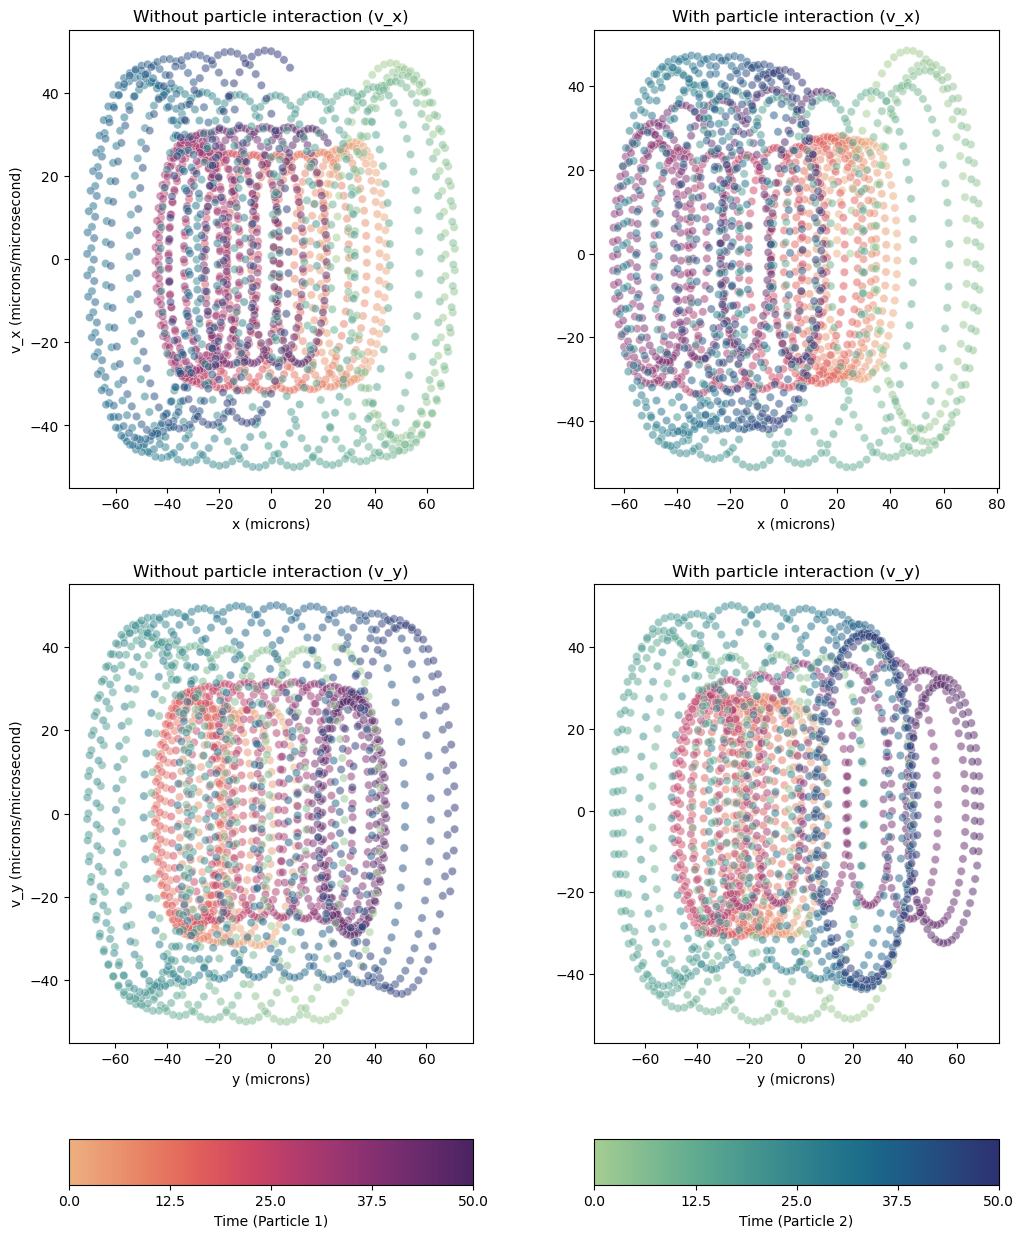
\includegraphics[width=.9\linewidth]{Project 3/figures/two_particles_v-vs-r.png}
    \caption{The phase-space plots for two particles. Upper row shows the velocity in the x plane as a function of x position and lower shows corresponding for y.}
    \label{fig:phase-space}
\end{figure}

\begin{figure}[h!]
    \centering
    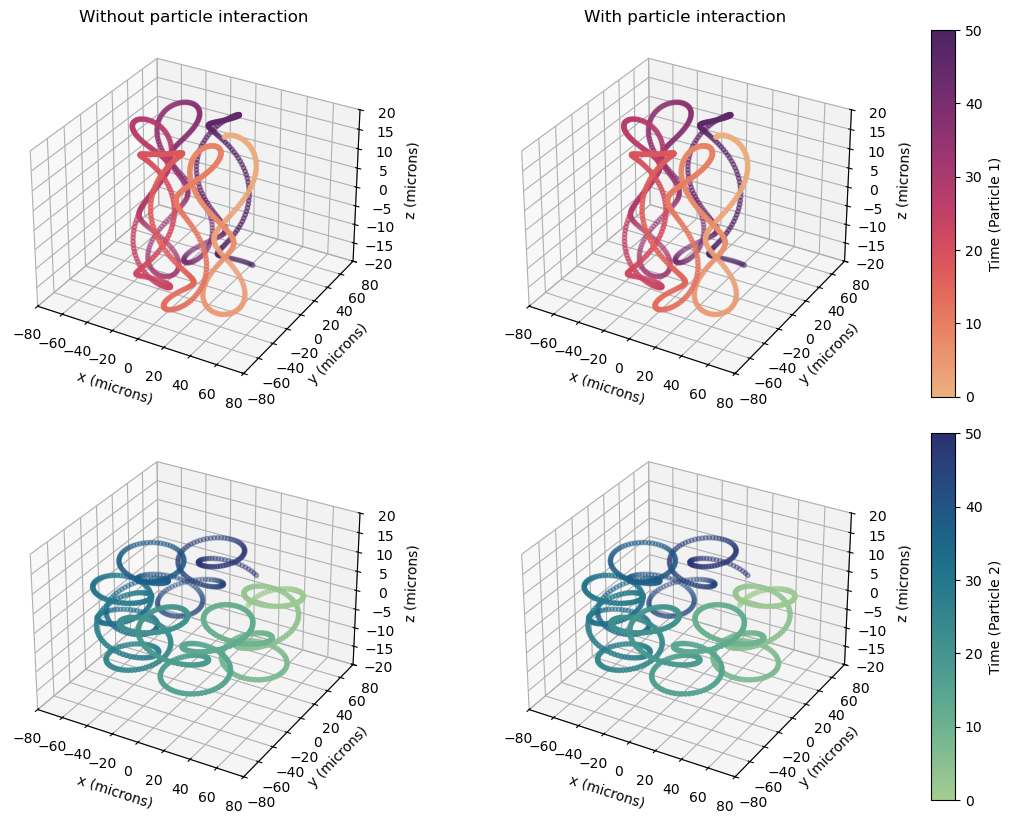
\includegraphics[width=.9\linewidth]{Project 3/figures/two_particles_3d.png}
    \caption{The particle position in 3d. The particles are displayed in separate plots for illustration proposes but are simulated in the same Penning trap simultaneously. }
    \label{fig:two_particles_3d}
\end{figure}

\end{document}
